\documentclass[tikz,border=10pt]{standalone}
\usepackage[T1]{fontenc}
\usepackage{lmodern}
\usepackage{amsmath}
\usepackage{graphicx}
\usetikzlibrary{arrows.meta,positioning,fit,calc,backgrounds}

\begin{document}
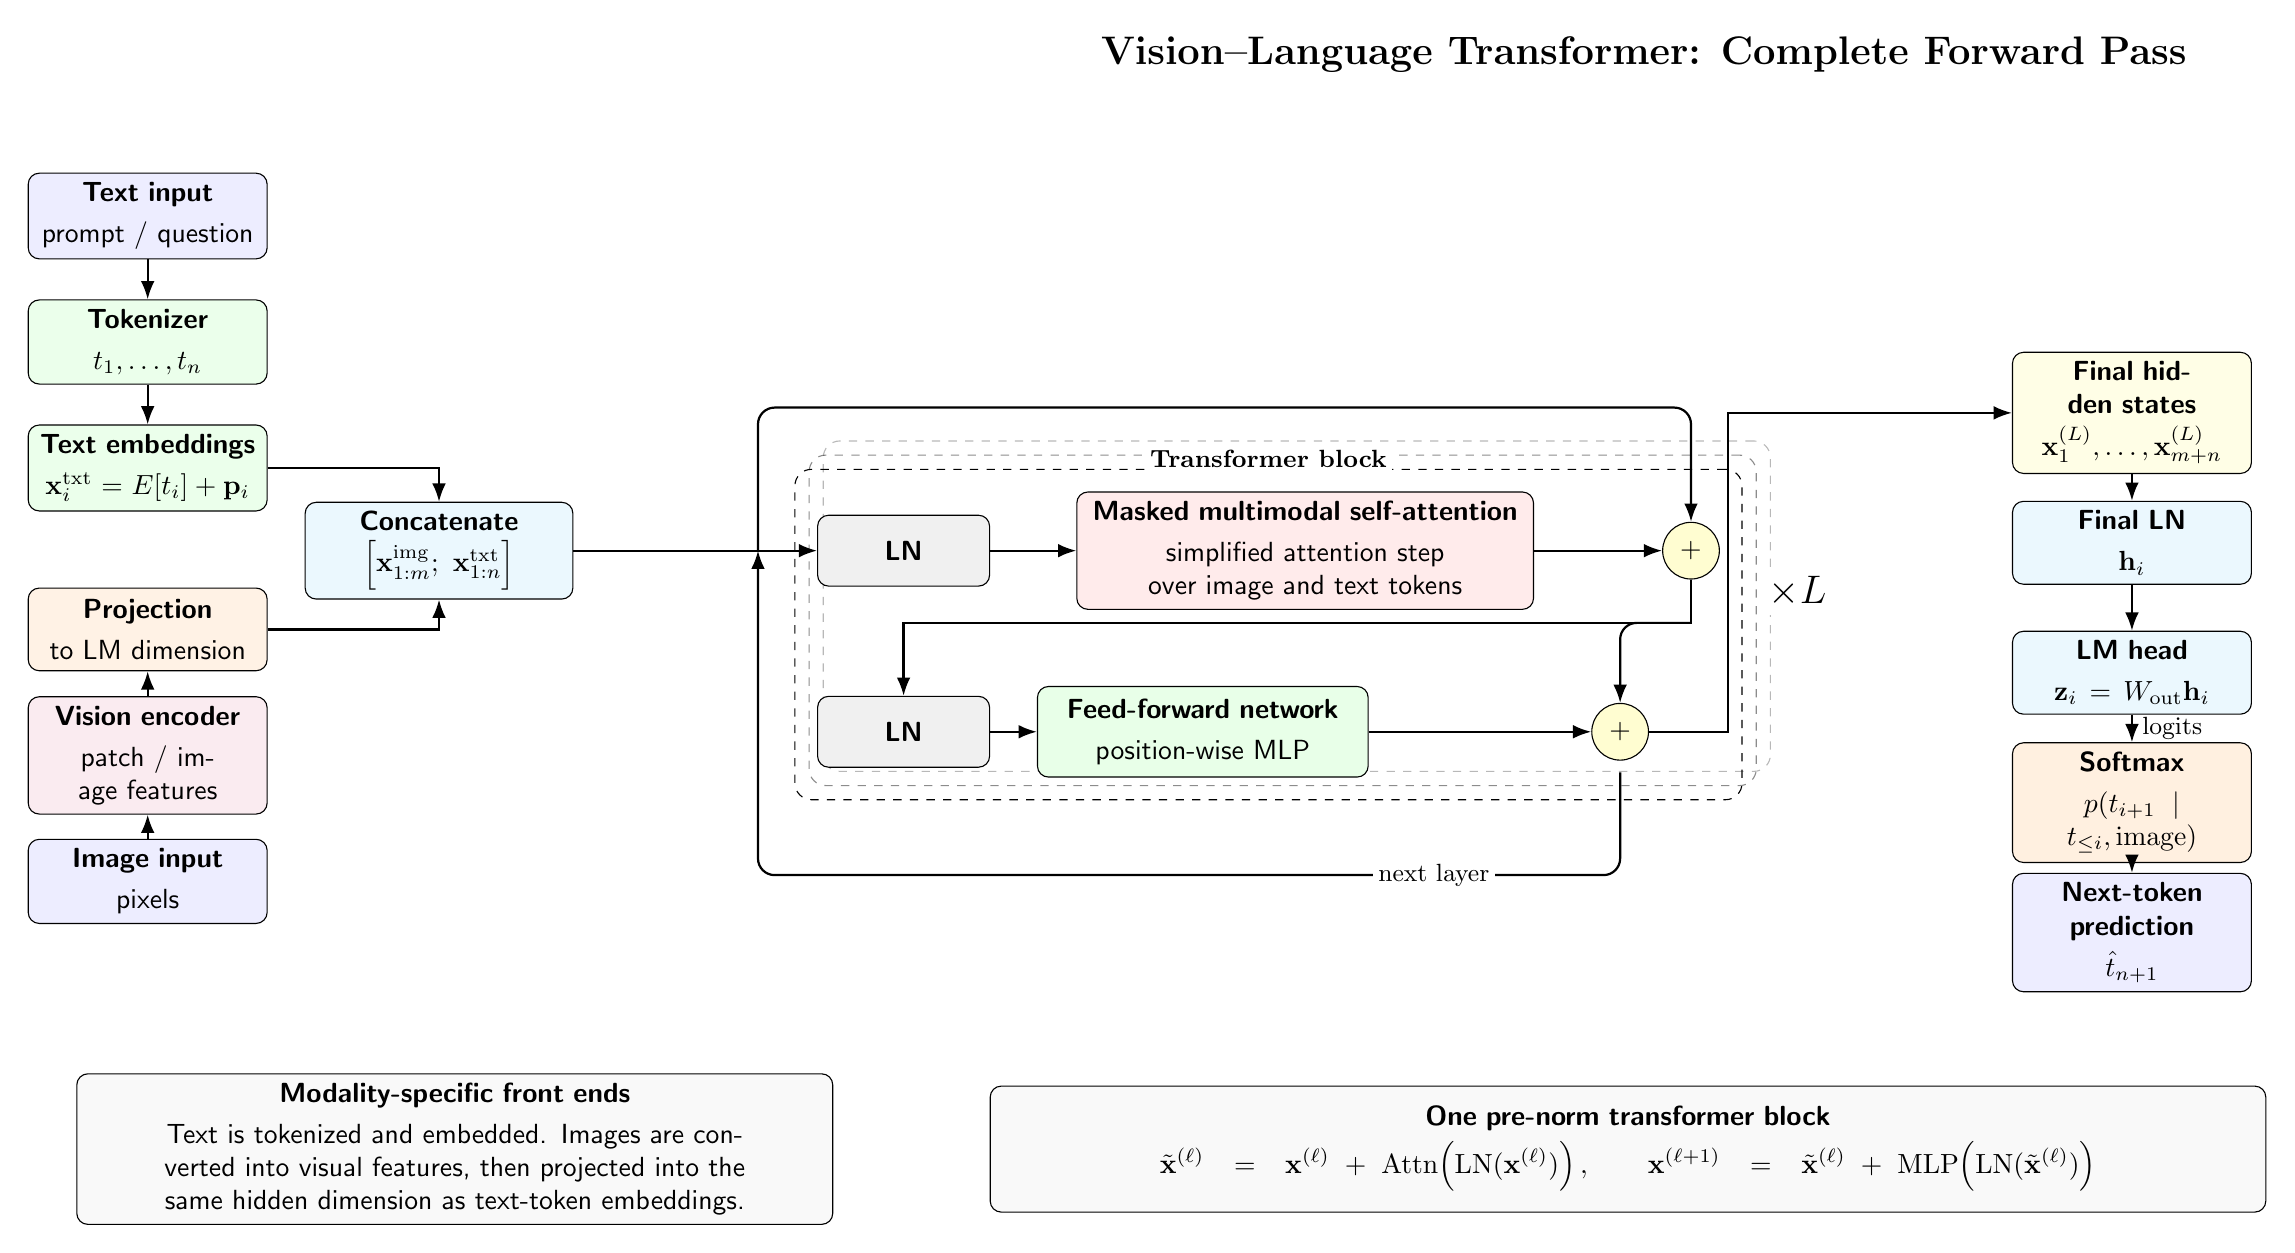
\begin{tikzpicture}[
    font=\sffamily,
    >=Latex,
    arrow/.style={->, thick},
    skiparrow/.style={->, thick, rounded corners=6pt},
    box/.style={
        draw,
        rounded corners=4pt,
        align=center,
        minimum height=1.05cm,
        minimum width=3.0cm,
        text width=2.8cm
    },
    widebox/.style={
        draw,
        rounded corners=4pt,
        align=center,
        minimum height=1.10cm,
        minimum width=3.9cm,
        text width=3.65cm
    },
    tinybox/.style={
        draw,
        rounded corners=4pt,
        align=center,
        minimum height=0.90cm,
        minimum width=2.1cm,
        text width=1.95cm
    },
    concatstyle/.style={
        draw,
        rounded corners=4pt,
        align=center,
        fill=cyan!8,
        minimum height=1.00cm,
        minimum width=3.4cm,
        text width=3.15cm
    },
    addbox/.style={
        circle,
        draw,
        fill=yellow!18,
        minimum size=0.72cm,
        inner sep=0pt,
        font=\bfseries
    },
    inputbox/.style={box, fill=blue!7},
    imagebox/.style={box, fill=purple!8},
    textbox/.style={box, fill=green!8},
    projbox/.style={box, fill=orange!10},
    normbox/.style={tinybox, fill=gray!12},
    attnbox/.style={
        draw,
        rounded corners=4pt,
        align=center,
        fill=red!8,
        minimum height=1.45cm,
        minimum width=5.8cm,
        text width=5.45cm
    },
    mlpbox/.style={
        draw,
        rounded corners=4pt,
        align=center,
        fill=green!9,
        minimum height=1.15cm,
        minimum width=4.2cm,
        text width=3.95cm
    },
    outbox/.style={box, fill=yellow!10},
    headbox/.style={box, fill=cyan!8},
    probbox/.style={box, fill=orange!12},
    dashedbox/.style={
        draw,
        dashed,
        rounded corners=6pt,
        inner sep=8pt
    }
]

% Title
\node[font=\bfseries\Large] (title) at (19.0,5.15)
{Vision--Language Transformer: Complete Forward Pass};

% ---------------------------------------------------------------------
% Modality-specific front ends
% ---------------------------------------------------------------------

% Text path, vertical stack: data flows downward
\node[inputbox] (textinput) at (0,3.1) {
\textbf{Text input}\\[1mm]
prompt / question
};

\node[textbox] (tokenizer) at (0,1.5) {
\textbf{Tokenizer}\\[1mm]
$t_1,\ldots,t_n$
};

\node[textbox] (textembed) at (0,-0.1) {
\textbf{Text embeddings}\\[1mm]
$\mathbf{x}^{\mathrm{txt}}_i
=
E[t_i]+\mathbf{p}_i$
};

% Image path, vertical stack: data flows upward
\node[inputbox] (imageinput) at (0,-5.35) {
\textbf{Image input}\\[1mm]
pixels
};

\node[imagebox] (visionencoder) at (0,-3.75) {
\textbf{Vision encoder}\\[1mm]
patch / image features
};

\node[projbox] (imageproj) at (0,-2.15) {
\textbf{Projection}\\[1mm]
to LM dimension
};

% Front-end arrows
\draw[arrow] (textinput.south) -- (tokenizer.north);
\draw[arrow] (tokenizer.south) -- (textembed.north);

\draw[arrow] (imageinput.north) -- (visionencoder.south);
\draw[arrow] (visionencoder.north) -- (imageproj.south);

% Concatenation / merged sequence
\node[concatstyle] (concat) at (3.7,-1.15) {
\textbf{Concatenate}\\[1mm]
$\left[
\mathbf{x}^{\mathrm{img}}_{1:m};\
\mathbf{x}^{\mathrm{txt}}_{1:n}
\right]$
};

% Arrows enter Concatenate through its upper and lower edges
\draw[arrow] (textembed.east) -- ++(1.0,0) -| (concat.north);
\draw[arrow] (imageproj.east) -- ++(1.0,0) -| (concat.south);

% ---------------------------------------------------------------------
% Transformer block
% First LN is aligned with Concatenate
% ---------------------------------------------------------------------

\node[normbox] (ln1) at (9.6,-1.15) {
\textbf{LN}
};

\node[attnbox] (attn) at (14.7,-1.15) {
\textbf{Masked multimodal self-attention}\\[1mm]
simplified attention step over image and text tokens
};

\node[addbox] (add1) at (19.6,-1.15) {$+$};

\node[normbox] (ln2) at (9.6,-3.45) {
\textbf{LN}
};

\node[mlpbox] (mlp) at (13.4,-3.45) {
\textbf{Feed-forward network}\\[1mm]
position-wise MLP
};

\node[addbox] (add2) at (18.7,-3.45) {$+$};

% ---------------------------------------------------------------------
% Output stack
% ---------------------------------------------------------------------

\node[outbox] (hidden) at (25.2,0.6) {
\textbf{Final hidden states}\\[1mm]
$\mathbf{x}^{(L)}_1,\ldots,\mathbf{x}^{(L)}_{m+n}$
};

\node[headbox] (finalln) at (25.2,-1.05) {
\textbf{Final LN}\\[1mm]
$\mathbf{h}_i$
};

\node[headbox] (lmhead) at (25.2,-2.70) {
\textbf{LM head}\\[1mm]
$\mathbf{z}_i
=
W_{\rm out}\mathbf{h}_i$
};

\node[probbox] (softmax) at (25.2,-4.35) {
\textbf{Softmax}\\[1mm]
$p(t_{i+1}\mid t_{\le i},\mathrm{image})$
};

\node[inputbox] (nexttoken) at (25.2,-6.00) {
\textbf{Next-token prediction}\\[1mm]
$\hat{t}_{n+1}$
};

% ---------------------------------------------------------------------
% Transformer-block arrows
% ---------------------------------------------------------------------

% Input to the transformer block
\coordinate (blockinput) at ($(ln1.west)+(-0.75,0)$);
\draw[arrow] (concat.east) -- (blockinput) -- (ln1.west);

% Attention path
\draw[arrow] (ln1.east) -- (attn.west);
\draw[arrow] (attn.east) -- (add1.west);

% First residual connection:
% x^(ell) bypasses LN + attention and enters Add 1.
% Raised higher so it no longer overlaps the Transformer block title.
\coordinate (resoneTop) at ($(add1.north)+(0,1.45)$);
\draw[skiparrow]
    (blockinput)
    |- (resoneTop)
    -- (add1.north);

% Output of Add 1 is \tilde{x}^{(ell)}.
% It goes both to the second LayerNorm and as a residual to Add 2.
\coordinate (afteraddone) at ($(add1.south)+(0,-0.55)$);

\draw[arrow]
    (add1.south)
    -- (afteraddone)
    -| (ln2.north);

% MLP path
\draw[arrow] (ln2.east) -- (mlp.west);
\draw[arrow] (mlp.east) -- (add2.west);

% Second residual connection:
% \tilde{x}^{(ell)} bypasses LN + MLP and enters Add 2.
\coordinate (restwoTop) at ($(add2.north)+(0,0.55)$);
\draw[skiparrow]
    (afteraddone)
    -| (restwoTop)
    -- (add2.north);

% Output of the final transformer block goes into the vertical output stack
\draw[arrow] (add2.east) -- ++(1.0,0) |- (hidden.west);

% Arrows inside the output stack
\draw[arrow] (hidden.south) -- (finalln.north);
\draw[arrow] (finalln.south) -- (lmhead.north);
\draw[arrow] (lmhead.south) -- node[right, font=\small] {logits} (softmax.north);
\draw[arrow] (softmax.south) -- (nexttoken.north);

% ---------------------------------------------------------------------
% Repeated transformer block visual cue
% ---------------------------------------------------------------------

\begin{pgfonlayer}{background}

% Back copies to suggest that the whole transformer block is stacked L times
\node[
    draw,
    dashed,
    rounded corners=6pt,
    inner sep=8pt,
    xshift=0.36cm,
    yshift=0.36cm,
    opacity=0.28
] (blockcopytwo) [fit=(ln1)(attn)(add1)(ln2)(mlp)(add2)] {};

\node[
    draw,
    dashed,
    rounded corners=6pt,
    inner sep=8pt,
    xshift=0.18cm,
    yshift=0.18cm,
    opacity=0.45
] (blockcopyone) [fit=(ln1)(attn)(add1)(ln2)(mlp)(add2)] {};

% Front block
\node[
    draw,
    dashed,
    rounded corners=6pt,
    inner sep=8pt
] (blockfit) [fit=(ln1)(attn)(add1)(ln2)(mlp)(add2)] {};

% Label above block
\node[
    font=\bfseries\small,
    fill=white,
    inner sep=2pt
] at ($(blockfit.north)+(0,0.12)$)
{Transformer block};

% Large repetition label
\node[
    font=\bfseries\Large,
    fill=white,
    inner sep=3pt
] at ($(blockfit.east)+(0.70,0.55)$)
{$\times L$};

\end{pgfonlayer}

% Loop-back arrow showing that the output of one layer becomes
% the input to the next layer.
% The loop now travels below the transformer block.
\coordinate (layerout) at ($(add2.south)+(0,-0.15)$);
\coordinate (loopbottom) at ($(blockfit.south)+(0,-0.95)$);
\coordinate (loopin) at ($(blockinput)+(0,-0.95)$);

\draw[skiparrow]
    (layerout)
    -- (layerout |- loopbottom)
    -- (loopin |- loopbottom)
    -- (loopin)
    -- (blockinput);

\node[
    font=\small,
    fill=white,
    inner sep=2pt
] at ($(blockfit.south)+(2.1,-0.95)$)
{next layer};

% ---------------------------------------------------------------------
% Compact explanatory boxes underneath
% ---------------------------------------------------------------------

\node[
    draw,
    rounded corners=4pt,
    align=center,
    fill=gray!5,
    minimum width=9.6cm,
    text width=9.3cm,
    minimum height=1.6cm
] (frontendnote) at (3.9,-8.75) {
\textbf{Modality-specific front ends}\\[1mm]
Text is tokenized and embedded. Images are converted into visual features,
then projected into the same hidden dimension as text-token embeddings.
};

\node[
    draw,
    rounded corners=4pt,
    align=center,
    fill=gray!5,
    minimum width=16.2cm,
    text width=15.9cm,
    minimum height=1.6cm
] (blockformula) at (18.8,-8.75) {
\textbf{One pre-norm transformer block}\\[1mm]
$\displaystyle
\tilde{\mathbf{x}}^{(\ell)}
=
\mathbf{x}^{(\ell)}
+
\mathrm{Attn}\!\left(\mathrm{LN}(\mathbf{x}^{(\ell)})\right),
\qquad
\mathbf{x}^{(\ell+1)}
=
\tilde{\mathbf{x}}^{(\ell)}
+
\mathrm{MLP}\!\left(\mathrm{LN}(\tilde{\mathbf{x}}^{(\ell)})\right)
$
};

\end{tikzpicture}
\end{document}